

\documentclass[conference]{IEEEtran}
%e compiler may
% have to be run twice to clear warning/error messages.






% *** CITATION PACKAGES ***
%
%\usepackage{cite}
% cite.sty was written by Donald Arseneau
% V1.6 and later of IEEEtran pre-defines the format of the cite.sty package
% \cite{} output to follow that of IEEE. Loading the cite package will
% result in citation numbers being automatically sorted and properly
% "compressed/ranged". e.g., [1], [9], [2], [7], [5], [6] without using
% cite.sty will become [1], [2], [5]--[7], [9] using cite.sty. cite.sty's
% \cite will automatically add leading space, if needed. Use cite.sty's
% noadjust option (cite.sty V3.8 and later) if you want to turn this off.
% cite.sty is already installed on most LaTeX systems. Be sure and use
% version 4.0 (2003-05-27) and later if using hyperref.sty. cite.sty does
% not currently provide for hyperlinked citations.
% The latest version can be obtained at:
% http://www.ctan.org/tex-archive/macros/latex/contrib/cite/
% The documentation is contained in the cite.sty file itself.






% *** GRAPHICS RELATED PACKAGES ***
%
\ifCLASSINFOpdf
  % \usepackage[pdftex]{graphicx}
  % declare the path(s) where your graphic files are
  % \graphicspath{{../pdf/}{../jpeg/}}
  % and their extensions so you won't have to specify these with
  % every instance of \includegraphics
  % \DeclareGraphicsExtensions{.pdf,.jpeg,.png}
\else
  % or other class option (dvipsone, dvipdf, if not using dvips). graphicx
  % will default to the driver specified in the system graphics.cfg if no
  % driver is specified.
  % \usepackage[dvips]{graphicx}
  % declare the path(s) where your graphic files are
  % \graphicspath{{../eps/}}
  % and their extensions so you won't have to specify these with
  % every instance of \includegraphics
  % \DeclareGraphicsExtensions{.eps}
\fi
\usepackage[dvips]{graphicx}
\usepackage{listings}
\usepackage{color}
\usepackage{url}
% graphicx was written by David Carlisle and Sebastian Rahtz. It is
% required if you want graphics, photos, etc. graphicx.sty is already
% installed on most LaTeX systems. The latest version and documentation can
% be obtained at: 
% http://www.ctan.org/tex-archive/macros/latex/required/graphics/
% Another good source of documentation is "Using Imported Graphics in
% LaTeX2e" by Keith Reckdahl which can be found as epslatex.ps or
% epslatex.pdf at: http://www.ctan.org/tex-archive/info/
%
% latex, and pdflatex in dvi mode, support graphics in encapsulated
% postscript (.eps) format. pdflatex in pdf mode supports graphics
% in .pdf, .jpeg, .png and .mps (metapost) formats. Users should ensure
% that all non-photo figures use a vector format (.eps, .pdf, .mps) and
% not a bitmapped formats (.jpeg, .png). IEEE frowns on bitmapped formats
% which can result in "jaggedy"/blurry rendering of lines and letters as
% well as large increases in file sizes.
%
% You can find documentation about the pdfTeX application at:
% http://www.tug.org/applications/pdftex





% *** MATH PACKAGES ***
%
%\usepackage[cmex10]{amsmath}
% A popular package from the American Mathematical Society that provides
% many useful and powerful commands for dealing with mathematics. If using
% it, be sure to load this package with the cmex10 option to ensure that
% only type 1 fonts will utilized at all point sizes. Without this option,
% it is possible that some math symbols, particularly those within
% footnotes, will be rendered in bitmap form which will result in a
% document that can not be IEEE Xplore compliant!
%
% Also, note that the amsmath package sets \interdisplaylinepenalty to 10000
% thus preventing page breaks from occurring within multiline equations. Use:
%\interdisplaylinepenalty=2500
% after loading amsmath to restore such page breaks as IEEEtran.cls normally
% does. amsmath.sty is already installed on most LaTeX systems. The latest
% version and documentation can be obtained at:
% http://www.ctan.org/tex-archive/macros/latex/required/amslatex/math/

\lstset{ %
language=C++,                % choose the language of the code
basicstyle=\tiny,       % the size of the fonts that are used for the code
%numbers=left,                   % where to put the line-numbers
numberstyle=\tiny,      % the size of the fonts that are used for the line-numbers
keywordstyle=\color{black}\bfseries,
stepnumber=1,                   % the step between two line-numbers. If it is 1 each line will be numbered
numbersep=5pt,                  % how far the line-numbers are from the code
backgroundcolor=\color{white},  % choose the background color. You must add \usepackage{color}
showspaces=false,               % show spaces adding particular underscores
showstringspaces=false,         % underline spaces within strings
showtabs=false,                 % show tabs within strings adding particular underscores
frame=single,                   % adds a frame around the code
tabsize=2,              % sets default tabsize to 2 spaces
captionpos=b,                   % sets the caption-position to bottom
breaklines=true,        % sets automatic line breaking
breakatwhitespace=false,    % sets if automatic breaks should only happen at whitespace
escapeinside={\%}{)}          % if you want to add a comment within your code
}





\usepackage{algorithmic}
\usepackage{algorithm}


% *** ALIGNMENT PACKAGES ***
%
%\usepackage{array}
% Frank Mittelbach's and David Carlisle's array.sty patches and improves
% the standard LaTeX2e array and tabular environments to provide better
% appearance and additional user controls. As the default LaTeX2e table
% generation code is lacking to the point of almost being broken with
% respect to the quality of the end results, all users are strongly
% advised to use an enhanced (at the very least that provided by array.sty)
% set of table tools. array.sty is already installed on most systems. The
% latest version and documentation can be obtained at:
% http://www.ctan.org/tex-archive/macros/latex/required/tools/


%\usepackage{mdwmath}
%\usepackage{mdwtab}
% Also highly recommended is Mark Wooding's extremely powerful MDW tools,
% especially mdwmath.sty and mdwtab.sty which are used to format equations
% and tables, respectively. The MDWtools set is already installed on most
% LaTeX systems. The lastest version and documentation is available at:
% http://www.ctan.org/tex-archive/macros/latex/contrib/mdwtools/


% IEEEtran contains the IEEEeqnarray family of commands that can be used to
% generate multiline equations as well as matrices, tables, etc., of high
% quality.


%\usepackage{eqparbox}
% Also of notable interest is Scott Pakin's eqparbox package for creating
% (automatically sized) equal width boxes - aka "natural width parboxes".
% Available at:
% http://www.ctan.org/tex-archive/macros/latex/contrib/eqparbox/





% *** SUBFIGURE PACKAGES ***
%\usepackage[tight,footnotesize]{subfigure}
% subfigure.sty was written by Steven Douglas Cochran. This package makes it
% easy to put subfigures in your figures. e.g., "Figure 1a and 1b". For IEEE
% work, it is a good idea to load it with the tight package option to reduce
% the amount of white space around the subfigures. subfigure.sty is already
% installed on most LaTeX systems. The latest version and documentation can
% be obtained at:
% http://www.ctan.org/tex-archive/obsolete/macros/latex/contrib/subfigure/
% subfigure.sty has been superceeded by subfig.sty.



%\usepackage[caption=false]{caption}
%\usepackage[font=footnotesize]{subfig}
% subfig.sty, also written by Steven Douglas Cochran, is the modern
% replacement for subfigure.sty. However, subfig.sty requires and
% automatically loads Axel Sommerfeldt's caption.sty which will override
% IEEEtran.cls handling of captions and this will result in nonIEEE style
% figure/table captions. To prevent this problem, be sure and preload
% caption.sty with its "caption=false" package option. This is will preserve
% IEEEtran.cls handing of captions. Version 1.3 (2005/06/28) and later 
% (recommended due to many improvements over 1.2) of subfig.sty supports
% the caption=false option directly:
%\usepackage[caption=false,font=footnotesize]{subfig}
%
% The latest version and documentation can be obtained at:
% http://www.ctan.org/tex-archive/macros/latex/contrib/subfig/
% The latest version and documentation of caption.sty can be obtained at:
% http://www.ctan.org/tex-archive/macros/latex/contrib/caption/




% *** FLOAT PACKAGES ***
%
%\usepackage{fixltx2e}
% fixltx2e, the successor to the earlier fix2col.sty, was written by
% Frank Mittelbach and David Carlisle. This package corrects a few problems
% in the LaTeX2e kernel, the most notable of which is that in current
% LaTeX2e releases, the ordering of single and double column floats is not
% guaranteed to be preserved. Thus, an unpatched LaTeX2e can allow a
% single column figure to be placed prior to an earlier double column
% figure. The latest version and documentation can be found at:
% http://www.ctan.org/tex-archive/macros/latex/base/



%\usepackage{stfloats}
% stfloats.sty was written by Sigitas Tolusis. This package gives LaTeX2e
% the ability to do double column floats at the bottom of the page as well
% as the top. (e.g., "\begin{figure*}[!b]" is not normally possible in
% LaTeX2e). It also provides a command:
%\fnbelowfloat
% to enable the placement of footnotes below bottom floats (the standard
% LaTeX2e kernel puts them above bottom floats). This is an invasive package
% which rewrites many portions of the LaTeX2e float routines. It may not work
% with other packages that modify the LaTeX2e float routines. The latest
% version and documentation can be obtained at:
% http://www.ctan.org/tex-archive/macros/latex/contrib/sttools/
% Documentation is contained in the stfloats.sty comments as well as in the
% presfull.pdf file. Do not use the stfloats baselinefloat ability as IEEE
% does not allow \baselineskip to stretch. Authors submitting work to the
% IEEE should note that IEEE rarely uses double column equations and
% that authors should try to avoid such use. Do not be tempted to use the
% cuted.sty or midfloat.sty packages (also by Sigitas Tolusis) as IEEE does
% not format its papers in such ways.





% *** PDF, URL AND HYPERLINK PACKAGES ***
%
%\usepackage{url}
% url.sty was written by Donald Arseneau. It provides better support for
% handling and breaking URLs. url.sty is already installed on most LaTeX
% systems. The latest version can be obtained at:
% http://www.ctan.org/tex-archive/macros/latex/contrib/misc/
% Read the url.sty source comments for usage information. Basically,
% \url{my_url_here}.





% *** Do not adjust lengths that control margins, column widths, etc. ***
% *** Do not use packages that alter fonts (such as pslatex).         ***
% There should be no need to do such things with IEEEtran.cls V1.6 and later.
% (Unless specifically asked to do so by the journal or conference you plan
% to submit to, of course. )


% correct bad hyphenation here
\hyphenation{op-tical net-works semi-conduc-tor}


\begin{document}
%
% paper title
% can use linebreaks \\ within to get better formatting as desired
\title{Frequent item set mining on modern multi-core architectures}


% author names and affiliations
% use a multiple column layout for up to three different
% affiliations
\author{\IEEEauthorblockN{Rejith George Joseph \\ Girish Ravunnikutty \\ Rakesh Nair \\ and Ajith Kumar Vasanthakumar}
\IEEEauthorblockA{University of Florida\\
rjoseph, girishr raknair07 @ufl.edu}}


% conference papers do not typically use \thanks and this command
% is locked out in conference mode. If really needed, such as for
% the acknowledgment of grants, issue a \IEEEoverridecommandlockouts
% after \documentclass

% for over three affiliations, or if they all won't fit within the width
% of the page, use this alternative format:
% 
%\author{\IEEEauthorblockN{Michael Shell\IEEEauthorrefmark{1},
%Homer Simpson\IEEEauthorrefmark{2},
%James Kirk\IEEEauthorrefmark{3}, 
%Montgomery Scott\IEEEauthorrefmark{3} and
%Eldon Tyrell\IEEEauthorrefmark{4}}
%\IEEEauthorblockA{\IEEEauthorrefmark{1}School of Electrical and Computer Engineering\\
%Georgia Institute of Technology,
%Atlanta, Georgia 30332--0250\\ Email: see http://www.michaelshell.org/contact.html}
%\IEEEauthorblockA{\IEEEauthorrefmark{2}Twentieth Century Fox, Springfield, USA\\
%Email: homer@thesimpsons.com}
%\IEEEauthorblockA{\IEEEauthorrefmark{3}Starfleet Academy, San Francisco, California 96678-2391\\
%Telephone: (800) 555--1212, Fax: (888) 555--1212}
%\IEEEauthorblockA{\IEEEauthorrefmark{4}Tyrell Inc., 123 Replicant Street, Los Angeles, California 90210--4321}}




% use for special paper notices
%\IEEEspecialpapernotice{(Invited Paper)}




% make the title area
\maketitle


\begin{abstract}
%\boldmath
The abstract goes here.
\end{abstract}
% IEEEtran.cls defaults to using nonbold math in the Abstract.
% This preserves the distinction between vectors and scalars. However,
% if the conference you are submitting to favors bold math in the abstract,
% then you can use LaTeX's standard command \boldmath at the very start
% of the abstract to achieve this. Many IEEE journals/conferences frown on
% math in the abstract anyway.

% no keywords




% For peer review papers, you can put extra information on the cover
% page as needed:
% \ifCLASSOPTIONpeerreview
% \begin{center} \bfseries EDICS Category: 3-BBND \end{center}
% \fi
%
% For peerreview papers, this IEEEtran command inserts a page break and
% creates the second title. It will be ignored for other modes.
\IEEEpeerreviewmaketitle



\section{Introduction}

\section{Preliminaries}

\subsection{Frequent item set mining}

\begin{algorithm}\caption{Apriori Algorithm}\label{alg:apriori}
  \begin{algorithmic}[1]
	\STATE \texttt{candidate\_items = items}
	\STATE \texttt{K = 1}
	\WHILE {candidate\_items != empty}
	    \STATE \texttt{frequent\_items = count\_frequent\_items(candidate\_items)}
			\STATE \texttt{K = K + 1}
	    \STATE \texttt {candidate\_items = generate\_candidate\_items(frequent\_items, K)}
    \ENDWHILE
  \end{algorithmic}
\end{algorithm}



\subsection{Related Work}
There have been studies in the past focussing on frequent itemset mining and various approaches to quicken the process on GPU.The work of Govindraju, Manocha et al.[] on stream mining of quantiles and frequencies on GPUs deal with sorting that forms a computationally intensive part of the algorithm to find frequencies.Their approach uses the color blending and texture mapping capabilities of the GPU for performing the comparison operations and comparitor mapping.Two implementations of the Apriori algorithm on GPU was done by Fang, Lu et al.[].They proposed a novel method of representing the transactions in the form of bitmaps.The bitmaps can be efficiently partioned into the SIMD processorsThey also put forward a method to efficiently perform time consuming operation of counting by implementing lookup.Another implementation they proposed involves representing itemsets as a trie structure to facilitate quick traversal.An intelligent approach of combining top-down and bottom up searches to expedite the search was put forward by Sivanandam, et al [] 

\subsection{Java Fork/join framework}
Fork/Join~\cite{bib:java} is a lightweight task framework included in $JSR166y$~\cite{bib:jsr}, introduced as part of the Java 7~\cite{bib:jdk7} platform. The Fork/Join framework aims at providing a support for parallel programming by way of splitting a task into smaller tasks, which are performed in parallel, waiting for these tasks to complete and then composing the final result out of the intermediate results.

Fork/Join employs a simple and highly efficient design technique for obtaining good parallel performance. The algorithms employing Fork/Join are very similar to the familiar divide-and-conquer algorithms. Listing~\ref{list:forkjoin} shows typical Fork/Join algorithm. 

\begin{lstlisting}[caption={Typical Fork/Join algorithm}, label=list:forkjoin]
Result solve (Problem problem) 
{
   if( problem is small enough)
   {
	    compute the solution
	 }		 
	 else
	 {
	    split the program into small, independent parts
			fork new subtask to solve each independent part
			join all the subtasks
			compose a result from all the subtasks
	 }
}
\end{lstlisting}


Fork/Join algorithms are recursive by nature and involve splitting the task into subtasks until they are small enough to be solved sequentially. The $fork$ operation spawns a new parallel fork/join subtask. The $join$ operation causes the parent task to wait till all the forked subtasks have completed execution, where after it merges the results of the subtasks. A high level view of Fork/Join architecture is shown in Figure~\ref{fig:forkjoin}.

\begin{figure}[!t]
\centering
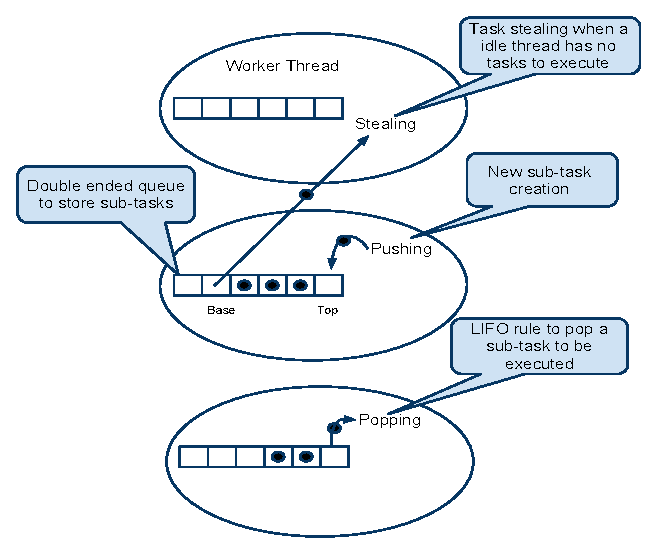
\includegraphics[width=2.5in]{forkjoin.eps}
\caption{Fork/Join schematic}
\label{fig:forkjoin}
\end{figure}

The Fork/Join framework can be implemented in a number of ways. The use of raw threads is an option. $Threads.start()$ and $Threads.join()$ will provide essentially a similar functionality. However this approach might result in the creation of a very large number of threads in the JVM, almost half of which will spend their entire time waiting for subtasks to complete. Hence this is not a good approach, especially since threads are expensive to create and use up a lot of memory. Some of the salient features of Fork/Join framework are

\begin{itemize}
\item{In Fork/Join program a pool of threads is maintained. These threads are assigned tasks to perform. Ideally the number of these threads will be equal to the number of available processors in a system with each thread being mapped to a single CPU.}
\item{A Task object needs to be created which the threads created recursively utilize.  A granularity parameter, which is algorithm dependent, needs to be identified, which forms the basis for ending any further creation of subtask and will cause an intermediate result to be generated.}
\item{Each worker thread maintains a double-ended queue to store its tasks. This queue performs both FIFO push and pop and LIFO Take operations. Every time a subtask is generated it is pushed into the queue. The worker threads process these tasks in a LIFO manner. When a thread has no task of its own to execute, it attempts to obtain a task from the queue of a random thread, using FIFO rule. This feature is called $Work-Stealing$.}
\item{When a worker thread encounters a join operation, it completes all the tasks until the target task is completed.}
\end{itemize}


\subsection{ OpenCL device architecture} \label{sec:gpuArch}

In this paper, we use GPUs and multi core CPUs as OpenCL~\cite{bib:ocl} devices. GPU is a dedicated computing device to address problems that have high arithmetic intensity i.e. high ratio of arithmetic operations to memory operations. Each of the GPU cores has a SIMT (Single Instruction Multiple Thread) architecture. The core of a GPU has a small cache and limited flow of control - both of these take up most of the transistors in a CPU whereas in a GPU, more transistors are used up for computing cores.

Parallel portions of an application are expressed as device kernels which run on many threads. GPU threads are extremely lightweight and the creation overhead is very little. The scheduling is done by the hardware unlike the operating system in a CPU. A typical GPU needs hundreds of threads for full utilization of hardware where as CPU can be saturated with only a few threads.

ATI (Owned by AMD) and NVIDIA are the leading vendors that provide GPUs with general purpose computing capabilities. NVIDIA provides the Compute Unified Device Architecture (CUDA) Framework with a new parallel programming model and Instruction Set Architecture to leverage the capabilities of the massive parallel computing hardware in NVIDIA GPUs. CUDA framework provides an extended C application programming interface and a run time library which enables the access and control of devices from the host. Similarly AMD provides ATI stream technology that enable AMD CPUs and GPUs to accelerate applications.

OpenCL (Open Computing Language) is an open royalty-free standard to write parallel programs that execute across heterogeneous computing environment consisting of CPUs, GPUs. OpenCL framework provides a ISO C99 based language for writing portable code that executes on heterogeneous platforms. NVIDIA provide openCL drivers for their GPUs and AMD provides for the CPUs and ATI GPUs.

An OpenCL device is identified as a collection of compute units. Each compute unit can contain many Processing Elements (PEs). OpenCL program executes in two parts: Kernels that execute on OpenCL devices and a host program that executes on the host. The instance of the kernel that is executing on a compute unit is called work-item. Work-items are organized into work groups Work-items in a work-group executes the same code in SIMD fashion on all the processing elements of a compute unit. Each work item in a work group has a unique ID and the work-groups has a global unique ID. In NVIDIA CUDA framework, work-items are identified as threads and work-group as blocks. The application running on the hosts uses OpenCL APIs to control the execution of kernels on devices. OpenCL provides a command queue interface to coordinate execution of kernels on the devices from the host. The host places kernel execution, memory transfer and synchronization commands into the command queue and are then scheduled to execute on the devices.

Work items executing an OpenCL kernel has access to four distinct memory hierarchies.
\begin{itemize}
\item{Global Memory: All the work-items in all work-roups has read and write access to this memory. Host can read and write to global memory
through memory commands placed on command queue. In a GPU, Global memory is implemented as DRAM. Hence the access latency is high. In NVIDIA GPUs, peak read performance occurs when all the work items access continuous global memory locations. This is known as coalesced memory access and is shown in Figure~\ref{fig:coalesced}.} Non-coalesced access is shown in Figure~\ref{fig:noncoalesced}
\item{Constant Memory: Part of the global memory that is read only to all work-items in all work-groups. Some devices provide fast cached access to constant memory. The memory is allocated and data is copied by the host.}
\item{Local Memory: The memory region local to a work-group, shared by all the work-items in that work-group. OpenCL devices like NVIDIA and ATI GPUs provide dedicated local memory on the device which is as fast as registers. In some other devices local memory is mapped to global memory. in NVIDIA GPUs, local memory is referred as shared memory. Shared memory is implemented as banks. When multiple work items (threads) in a work group (block) access the same bank, bank conflicts occur which results in the serialization of access.} 
\item{Private Memory: The memory region private to a work item. These are mostly hardware registers. In some devices like NVIDIA GPU excessive use of private memory results in register spilling to global memory which in turn degrades the performance. Host cannot read and write to local or private memories.}
\end{itemize}

\begin{figure}[!t]
\centering
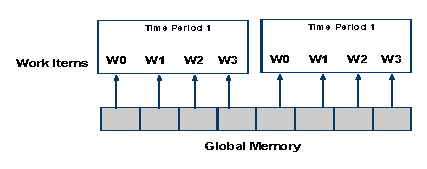
\includegraphics[width=2.5in]{coalesced.eps}
\caption{Coalesced Global Memory Access}
\label{fig:coalesced}
\end{figure}


\begin{figure}[!t]
\centering
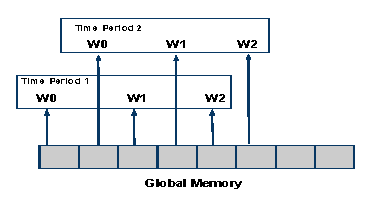
\includegraphics[width=2.5in]{noncoalesced.eps}
\caption{Non-Coalesced Global Memory Access}
\label{fig:noncoalesced}
\end{figure}

A high level view of OpenCL device architecture is shown in Figure~\ref{fig:computeDevice}.

\begin{figure}[!t]
\centering
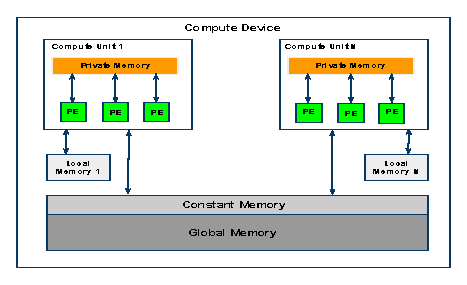
\includegraphics[width=2.5in]{computedevice.eps}
\caption{OpenCL compute device}
\label{fig:computeDevice}
\end{figure}

OpenCL provides two levels of synchronization
\begin{enumerate}
\item{Synchronization of work-items in a work group: This is a barrier synchronization which ensures all the work-items execute the barrier before proceeding to execution beyond the barrier.}
\item{Synchronization between commands enqueued in a command queue: This ensures that all the commands queued before the barrier have finished execution and the resulting memory is visible to the commands after the barrier before they begin execution.}
\end{enumerate}

\section{Parallel Apriori Algorithm}
As mentioned before, $Apriori$ algorithm works in iterations. Each iteration is dependent on the results (new candidate items) of the previous iteration. Hence the iterations of the $Apriori$ algorithm cannot be parallelized. What we can parallelize is the computations done with in an iteration. In this paper, we focus on parallelizing the $count\_frequent\_items(candidate\_items)$ step of Algorithm~\ref{alg:apriori}. We developed Java fork/join and OpenCL kernels for counting. The $generate\_candidate\_items(frequent\_items,\ K)$ is done on CPU. The parallel $Apriori$ algorithm is depicted in Algorithm ~\ref{alg:papriori}. 

\begin{algorithm}\caption{Parallel Apriori Algorithm}\label{alg:papriori}
  \begin{algorithmic}[1]
	\STATE \texttt{candidate\_items = items}
	\STATE \texttt{K = 1}
	\WHILE {candidate\_items != empty}
	    \FORALL{candidate\_items in parallel} 
	        \STATE \texttt{frequent\_items = count\_frequent\_items(candidate\_items, min\_support)}
			\ENDFOR		 
			\STATE \texttt{K = K + 1}
	    \STATE \texttt {candidate\_items = generate\_candidate\_items(frequent\_items, K)}
    \ENDWHILE
  \end{algorithmic}
\end{algorithm}

\subsection{Parallelization issues}
For parallelizing an algorithm on a multi-core architecture, we need to address the following issues:

\subsection{Fork/Join implementation}
The $Apriori$ implementation in Java begins with the creation of a boolean two dimensional array, called $marketBasket$, of items and transactions. An entry $marketBasket[i][j]=1$, indicates that the item $i$ is present in transaction $j$ and the value zero indicates that the item is not present in that specific transaction. A $frequentItems$ array list will hold all the frequent items, of length $0 to K$ after the program execution completes. 

The program begins with the creation of a $ForkJoinPool$ object, which creates a worker thread pool to be utilized during parallel execution. The number of worker threads in the pool is equal to the number of CPU's present in the system. The next step is to obtain the candidates for the current iteration, and the function $generateCandidateSet()$ performs this task and stores all the candidate items in an arraylist, $candidates$. The program continues iteratively till the candidates $arraylist$ so generated is of size zero.

During each iteration we loop through the $candidates$ arraylist and generate the count for the item stored in it. A $CountTask$ object, which extends the $ForkJoinTask$ class, and contains the counting logic, is created during each iteration of the loop. The $invoke()$ function causes the counting operation for that specific item, to begin. The $invoke()$ transfers the control to the $compute()$ function in $CountTask$ class, which splits the transaction array into $n$ parts, where $n$ is the number of processor cores, and assigns the task of counting the specific item occurrences in this sub-array, to each of the n available worker threads.  This is done by invoking the $forkJoin()$ function present in the $RecursiveActions$ class and passing an array of tasks(in this case new $CountTask$ objects, each containing a subset of the initial transaction array for the specific object) as a parameter. Thus the counting of the occurrences of a specific item is performed in parallel by distributing the tasks between each of the available CPU cores. At the end of an iteration, the count hashmap will contain an entry for each of the items in the previously generated candidate set and a corresponding count value associated with it. 
We then loop through the count hashmap and remove all the items whose count is less than the user specified Support Count.  The resultant contents of the $count$ hashmap will be the frequent $K$ item set. The items are copied into the $frequentItems$ arraylist. These items are also copied into the $candidate$ arraylist and then used during the next iteration to generate the candidates for $K+1$ frequent items.


\subsection{OpenCL implementation using bitmap}
We present the bitmap based implementation of the $Apriori$ algorithm. The motivation behind using a bitmap is to reduce the memory requirements of the $Apriori$ algorithm. The data set for Frequent Itemset Mining is expressed in market basket format shown in Figure~\ref{fig:marketbasket}. Market basket is a $transaction\ X\ items$ matrix. We transform this representation to a $item\ X\ transaction$ bitmap as shown in Figure~\ref{fig:bitmap}. Item $A$ is present in transactions $T1,\ T2,\ T4$, item $B$ in transactions $T1,\ T3,\ T4$ and so on. We refer this bitmap as transaction bitmap. 
\begin{figure}[!t]
\centering
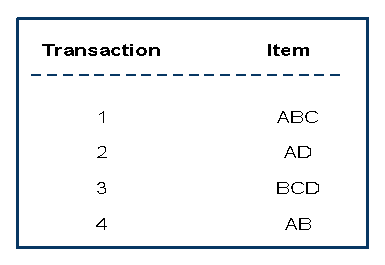
\includegraphics[width=1.5in]{marketbasket.eps}
\caption{Market Basket}
\label{fig:marketbasket}
\end{figure}

In each iteration, the transaction bitmap $tBitMap$ is copied to global memory of the device. We also keep a boolean array $isFrequent$ to keep track of the frequent items. i.e. $isFrequent[i] == true$ if $i^{th}$ candidate item set is frequent otherwise $false$. Once the kernel completes execution, the $isFrequent$  array is copied from device to the host. Listing~\ref{list:counting} shows the OpenCL kernel for counting frequent item sets.

\begin{figure}[!t]
\centering
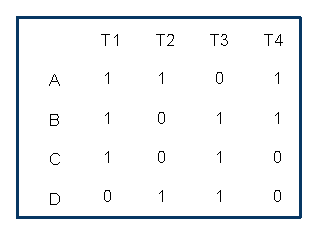
\includegraphics[width=1.5in]{bitmap.eps}
\caption{Bitmap Representation}
\label{fig:bitmap}
\end{figure}

The transaction bitmap is partitioned among the the work-groups such that each work-group performs counting for a group of item set. The work-items in a work-group scans the transaction bitmap corresponding to an item set and updates (atomic) a counter in local memory. The atomic update is required in a particular time-frame, all the work-items in a work-group scan the transaction bitmap corresponding to an item set. Currently we use a single integer element in the local memory. All the work-items perform atomic update of this element. This results in contention. One solution is to keep an array in local memory such that a group of work-items update a particular location. Then we perform a parallel reduce on this array to get the count. The count is then compared with the support value and the result is set in the $isFrequent$ array. Since the candidate item sets mapped to each work-group are independent, we do not need an atomic update in the global memory.

Another advantage of bitmap representation is efficient counting using bitwise operators. Work-items read the transactions corresponding to a candidate item set as an unsigned integer ($32$ bit) from the bitmap. This read from global memory is performed in coalesced pattern. We split the $32$ bit unsigned integer into two 16 bit unsigned integers. As shown in Figure~\ref{fig:lookup}, we maintain a look up table in the device constant memory that stores the number of $1's$ in $16$ bit unsigned integers. The look up table has $2^{16}$ one byte entires ($64$KB) which will fit into the constant memory of an OpenCL device.

\begin{figure}[!t]
\centering
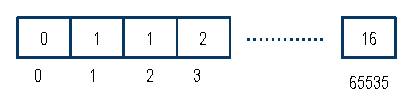
\includegraphics[width=2in]{lookuptable.eps}
\caption{16 bit look up table}
\label{fig:lookup}
\end{figure}


\begin{lstlisting}[caption={OpenCL Kernel for counting frequent item sets}, label=list:counting]
// lookup array in constant memory
// tBitMap array in global memory
// sCount in shared memory
// WIPWG - Work-items per work-group
// DPWI - Data per work-item
// IPWG - Items per work-group
// tx - work-item id
for (uint k = 0; k < IPWG; ++k) 
{
   uint count = 0;
   for (uint i = 0; i < DPWI; ++i) 
	 {	
       uint index = start + (i * WIPWG) + tx;
       uint val = (tBitMap[index]);
       ushort upval = (val & 0xffff0000) >> 16;
       ushort lowval = val & 0x0000ffff;
       count += lookup[upval] + lookup[lowval];
   }
   if (count)
      atom_add(sCount, count);
   barrier(CLK_LOCAL_MEM_FENCE);
   if (tx == 0) 
	 {	
      if (*sCount > support) 
		     isFrequent[start + k] = 1;
      *sCount = 0; 
   }
   barrier(CLK_LOCAL_MEM_FENCE);
}
\end{lstlisting}

The candidate generation step is done on CPU. In $Apriori$ algorithm a $K$ item set is a candidate if all the $K-1$ subsets are frequent. For efficient implementation, we use a trie data structure. A trie is created for the item sets. A trie is a directed prefix tree. Each node in the tree stores an item id.
A node at depth $K$, prefixing the path from root to the node represents a K item set. The nodes also store the indexes to the $isFrequent$ array to get the frequency. The index also points to the corresponding entry of the item set in the transaction bitmap. We generate the candidate item sets by traversing the trie. i.e. to generate $K$ item set from $K - 1$ item set, we traverse the trie till we reach the leaf node at level $K - 1$. Each item in the lead is joined with its right sibling to form a $K$ item set. The children of a node are kept in lexicographical sorted order on item id which ensures joining with right sibling generates a $K$ item set. Then we check if all the (K-1) item sets of this K item are frequent by traversing the trie. If its a candidate K-item set, the sibling is added as the child of the leaf node. A logical AND operation is performed between the corresponding entires in the transaction bitmap of the two items. This generation the K-transaction bitmap used for counting in next iteration.

Figure~\ref{fig:trie} shows generating $3$ item set from $2$ item set. The two item sets $AB$ and $AC$ are joined to form the three item set $ABC$. We do  logical AND operation of entries corresponding to $AB$ and $AC$ in the transaction bitmap to form the new transaction bitmap with entry $ABC$.


\begin{figure}[!t]
\centering
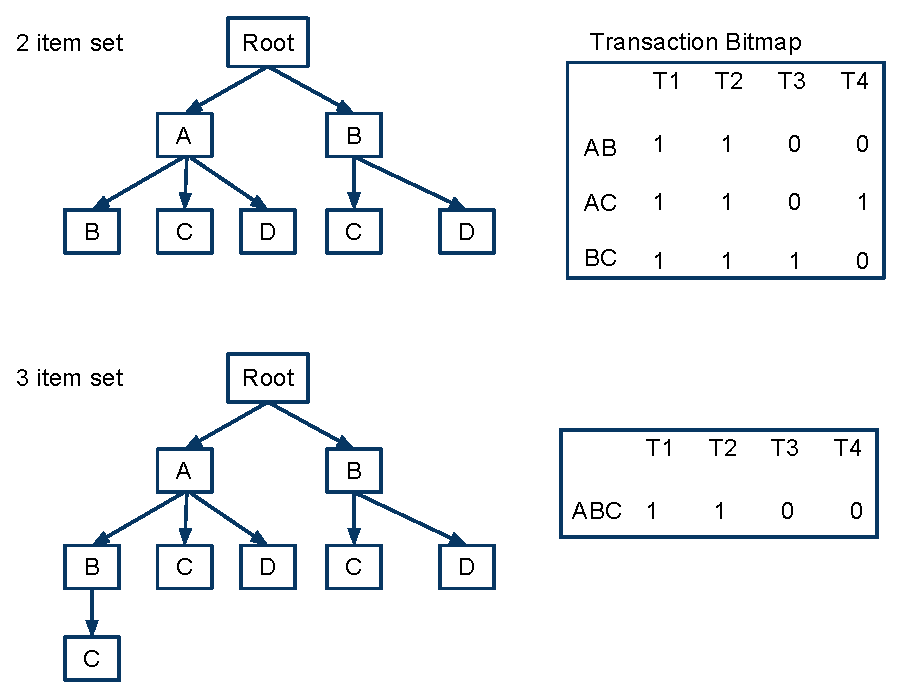
\includegraphics[width=3in]{trie.eps}
\caption{Generating 3 item set from 2 item set using trie}
\label{fig:trie}
\end{figure}


\section{Experimental Results}
\subsection{Data sets}
We used two data sets, $chess$ and $mushroom$ from Frequent Itemset Mining Dataset Repository (FIMI)~\cite{bib:fimi} to evaluate our $Apriori$ implementations. 
\subsection{Benchmark Machine}
We conducted our experiments on two different hardware configurations. All the machines run on $64bit$ Linux operating system. The OpenCL source code is compiled using $g++$ compiler.
\begin{enumerate}
\item{The machine with an NVIDIA FERMI Generation GeForce GTX 480 GPU clocked at $1.4GHz$. The GPU has $1.6	GB$ global memory and $48 KB$ local memory. It has $15$ compute units and each compute unit has $32$ processing elements resulting in a total of $480$ processor cores. The machine has a quad core Intel Xeon Processor clocked at $2.8GHz$ with $12GB$ RAM.}
\item{The machine with $8$ quad core AMD Opteron processors clocked at $3.6GHtz$ and 100GB RAM.}
\end{enumerate} 
\section{Conclusion and future work}


% An example of a floating figure using the graphicx package.
% Note that \label must occur AFTER (or within) \caption.
% For figures, \caption should occur after the \includegraphics.
% Note that IEEEtran v1.7 and later has special internal code that
% is designed to preserve the operation of \label within \caption
% even when the captionsoff option is in effect. However, because
% of issues like this, it may be the safest practice to put all your
% \label just after \caption rather than within \caption{}.
%
% Reminder: the "draftcls" or "draftclsnofoot", not "draft", class
% option should be used if it is desired that the figures are to be
% displayed while in draft mode.
%
%\begin{figure}[!t]
%\centering
%\includegraphics[width=2.5in]{myfigure}
% where an .eps filename suffix will be assumed under latex, 
% and a .pdf suffix will be assumed for pdflatex; or what has been declared
% via \DeclareGraphicsExtensions.
%\caption{Simulation Results}
%\label{fig_sim}
%\end{figure}

% Note that IEEE typically puts floats only at the top, even when this
% results in a large percentage of a column being occupied by floats.


% An example of a double column floating figure using two subfigures.
% (The subfig.sty package must be loaded for this to work.)
% The subfigure \label commands are set within each subfloat command, the
% \label for the overall figure must come after \caption.
% \hfil must be used as a separator to get equal spacing.
% The subfigure.sty package works much the same way, except \subfigure is
% used instead of \subfloat.
%
%\begin{figure*}[!t]
%\centerline{\subfloat[Case I]\includegraphics[width=2.5in]{subfigcase1}%
%\label{fig_first_case}}
%\hfil
%\subfloat[Case II]{\includegraphics[width=2.5in]{subfigcase2}%
%\label{fig_second_case}}}
%\caption{Simulation results}
%\label{fig_sim}
%\end{figure*}
%
% Note that often IEEE papers with subfigures do not employ subfigure
% captions (using the optional argument to \subfloat), but instead will
% reference/describe all of them (a), (b), etc., within the main caption.


% An example of a floating table. Note that, for IEEE style tables, the 
% \caption command should come BEFORE the table. Table text will default to
% \footnotesize as IEEE normally uses this smaller font for tables.
% The \label must come after \caption as always.
%
%\begin{table}[!t]
%% increase table row spacing, adjust to taste
%\renewcommand{\arraystretch}{1.3}
% if using array.sty, it might be a good idea to tweak the value of
% \extrarowheight as needed to properly center the text within the cells
%\caption{An Example of a Table}
%\label{table_example}
%\centering
%% Some packages, such as MDW tools, offer better commands for making tables
%% than the plain LaTeX2e tabular which is used here.
%\begin{tabular}{|c||c|}
%\hline
%One & Two\\
%\hline
%Three & Four\\
%\hline
%\end{tabular}
%\end{table}


% Note that IEEE does not put floats in the very first column - or typically
% anywhere on the first page for that matter. Also, in-text middle ("here")
% positioning is not used. Most IEEE journals/conferences use top floats
% exclusively. Note that, LaTeX2e, unlike IEEE journals/conferences, places
% footnotes above bottom floats. This can be corrected via the \fnbelowfloat
% command of the stfloats package.


% conference papers do not normally have an appendix


% use section* for acknowledgement


% trigger a \newpage just before the given reference
% number - used to balance the columns on the last page
% adjust value as needed - may need to be readjusted if
% the document is modified later
%\IEEEtriggeratref{8}
% The "triggered" command can be changed if desired:
%\IEEEtriggercmd{\enlargethispage{-5in}}

% references section

% can use a bibliography generated by BibTeX as a .bbl file
% BibTeX documentation can be easily obtained at:
% http://www.ctan.org/tex-archive/biblio/bibtex/contrib/doc/
% The IEEEtran BibTeX style support page is at:
% http://www.michaelshell.org/tex/ieeetran/bibtex/
%\bibliographystyle{IEEEtran}
% argument is your BibTeX string definitions and bibliography database(s)
%\bibliography{IEEEabrv,../bib/paper}
%
% <OR> manually copy in the resultant .bbl file
% set second argument of \begin to the number of references
% (used to reserve space for the reference number labels box)
\begin{thebibliography}{1}
\bibitem{bib:bitmap}
Wenbin Fang, Mian Lu, Xiangye Xiao, et.al., \emph{Frequent Itemset Mining on Graphics Processors}, 5th International Workshop on Data Management on New Hardware, June 2009.
\bibitem{bib:assocAlgos}
Rakesh Agrawal and Ramakrishnan Srikant, \emph{Fast algorithms for mining association rules}, VLDB, 1994.
\bibitem{bib:fimi}
http://fimi.cs.helsinki.fi, \emph{FIMI repository}
\bibitem{bib:ocl}
http://www.khronos.org/opencl, \emph{OpenCL 1.1 Specification}
\bibitem{bib:java}
Doug Lea, \emph{A Java Fork/Join Framework}
\bibitem{bib:jsr}
http://gee.cs.oswego.edu/dl/jsr166/dist/jsr166ydocs/, \emph{Concurrency JSR-166 Interest Site}, Doug Lea
\bibitem{bib:jdk7}
https://jdk7.dev.java.net/, \emph{Java 7}

\end{thebibliography}




% that's all folks
\end{document}


